The regime trichotomy --- isolated, blocked, alternating --- is the
organizing experimental fact of the synaptic-structure era. All three
were measured on the same cell (the e24 operating point
\(\beta=0.0046875,\ \tau_s=5000\)), same seeds, with the same
snapshot-based instrument \cite{synmem}; Figure~\ref{fig:regimes} shows
the end-state channel masses.

\paragraph{Isolated.} A single pattern trained to completion yields
clean winner selection: A-mass 0.290 / C-mass 0.026 (A-trained) or the
mirror (0.031 / 0.239, C-trained). The unchallenged group is pruned
away by budget normalization plus M4 selection.

\paragraph{Blocked.} Sequential blocks overwrite: BAC (20 A then 20 C)
ends at A-mass 0.068 / C-mass 0.137 --- the first block's mass is
removed by the second (unmodified substrate; the CLLA-era numbers in
\S\ref{sec:clla} reproduce the same shape under protection). BCA ends
at 0.234 / 0.105. Each blocked run drifts toward its final block's
trained endpoint (cos to its own endpoint 0.52--0.58) but lands between
the endpoints (both blocks leave residual mass).

\paragraph{Alternating.} Both groups remain driven, so neither is
pruned: end-state A-mass 0.239 / C-mass 0.162 --- both retained, no
overwrite. But the retained state is a superposition: it is neither a
mixture of the endpoints (best linear mixture leaves a 96\% residual)
nor a discriminator of the most recent episode (adjacent-state cosine
0.972 \(\to\) 0.990, \S\ref{sec:bottleneck}).

\paragraph{Causal decomposition.} SDE-B (doubling \(t_e\)) showed that
capacity is not the lever: the surplus feeds the dominant trace and
coexistence does not improve. SDE-C2 isolated passive decay as the
dominant eraser of the first block (decay-off preserves first-cohort
mass in 6/6 blocked runs). SDE-D showed the STDP \(a^-/a^+\)
asymmetry is secondary and context-dependent; the leading unresolved
residual mechanism was M2 reallocation (inference at the time, later
supported by the trace-partitioned M2 experiment, V2.3, which rescued
blocked-order collapse-class cells 6/6 by capacity-matched per-bucket
targets \cite{overview}).

\begin{quote}
\textbf{Demonstrated:} isolated \(\to\) winner selection; blocked
\(\to\) recency overwrite; alternating \(\to\) coexistence without
episode discrimination. The trichotomy reproduces at the protected
(CLLA) layer later (\S\ref{sec:clla}) and under all tested amendments
except the M2 partition, which was tested blocked-only.\\[1pt]
\textbf{Supported:} the shared per-neuron additive budget is the
interference medium; passive decay is the dominant eraser; budget
partition is the only measured lever improving blocked coexistence.
\end{quote}

\begin{figure}[t]
\centering
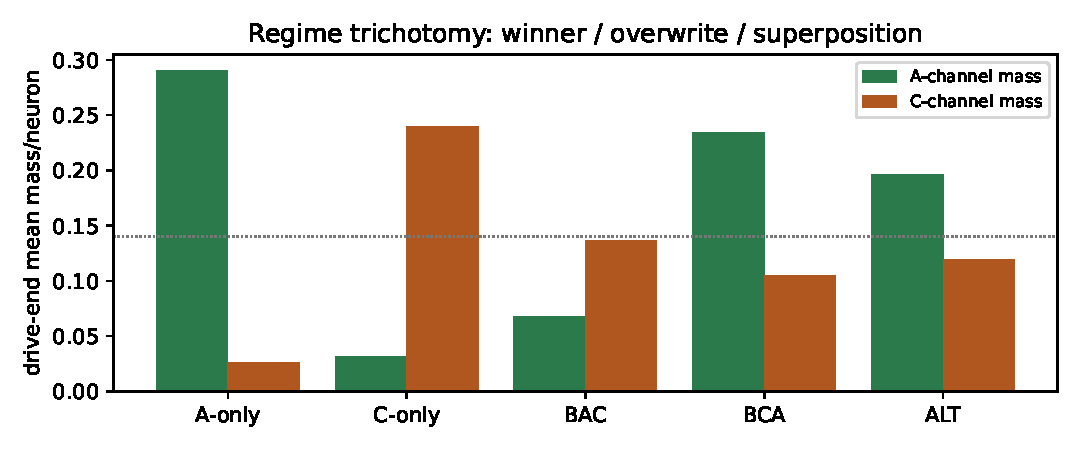
\includegraphics[width=\linewidth]{figures/fig5-regimes.pdf}
\caption{\textbf{Isolated vs.\ blocked vs.\ alternating synaptic
organization} (same cell, same seed; drive-end mean per-neuron channel mass; single-pattern and blocked bars recomputed from preserved
runs by the committed \texttt{papermass} instrument, reproducing the
audit table values at print precision; the alternating bar is the
e24-il run at the same 40-presentation convention (the audit's longer
40+40 alternating run reads 0.239/0.162 --- the same superposition, not
a mixture of the endpoints) \cite{synmem}). Isolated training selects
one channel group; blocked order
overwrites the earlier block; alternation retains both groups but as a
superposition that does not discriminate the most recent episode
\cite{synmem}.}
\label{fig:regimes}
\end{figure}